% don't remove the folling lines, and edit the defintion of \main if needed
\documentclass[../report.tex]{subfiles}
\providecommand{\main}{..}
\IfEq{\jobname}{\currfilebase}{\AtEndDocument{\biblio}}{}
% until here

%file for shortcuts

\newcommand{\nch}{\ensuremath{N_{\mathrm {ch}}\xspace}}
\newcommand{\Ncoll}{\ensuremath{N_{\mathrm {coll}}}}
\newcommand{\Npart}{\ensuremath{N_{\mathrm {part}}}}
\newcommand{\dNdeta}{\mathrm{d}N_\mathrm{ch}/\mathrm{d}\eta}
\newcommand{\snn}         {\ensuremath{\sqrt{s_{\mathrm {NN}}}}}
\newcommand{\kT}          {\ensuremath{k_{\mathrm {T}}}}

\newcommand{\pp}          {pp}
\newcommand{\pPb}         {pPb}
\newcommand{\pA}          {pA}
\newcommand{\PbPb}        {PbPb}
\newcommand{\AuAu}        {AuAu}
\newcommand{\CuCu}        {CuCu}
\newcommand{\pAu}         {pAu}
\newcommand{\dAu}         {dAu}
\newcommand{\lsim}        {\,{\buildrel < \over {_\sim}}\,}
\newcommand{\gsim}        {\,{\buildrel > \over {_\sim}}\,}
\newcommand{\co}[1]       {\relax}
\newcommand{\nl}          {\newline}
\newcommand{\el}          {\\\hline\\[-0.4cm]}
\usepackage{amsmath}
\usepackage{units}

\emergencystretch=1em
\raggedbottom

\begin{document}

\section{Emergence of Hot and Dense QCD in Small Systems}

\subsection{Historic overview}
% Comments wrt initial LHC program
% Table (-> Constantin, Naghmeh)

\begin{table}[h!]
\begin{center}
  \small
  \begin{tabular}{p{3.9cm}|p{2.7cm}|p{2.7cm}|p{2.6cm}| p{1.7cm} }
    Observable or effect                 & PbPb                                          & pPb (high mult.)                  & pp (high mult.)                         & Refs.\\
    \hline
    \hline
    Low $\pT$ spectra (``radial flow'')  & yes                                             & yes                                & yes                            & \cite{Abelev:2012wca,Abelev:2013vea,Chatrchyan:2013eya,Chatrchyan:2012qb,Andrei:2014vaa,Abelev:2013haa,Acharya:2017dmc,Adam:2016bpr,Adam:2015vsf,Adam:2017zbf} \el
    Intermed.\ $\pT$ (``recombination'') & yes                                             & yes                                & yes                            & \cite{Andrei:2014vaa,Abelev:2013xaa,Abelev:2013haa,Abelev:2014uua,Khachatryan:2016yru,Adam:2015jca,Adam:2016dau,Adam:2017zbf} \el
    Particle ratios                      & GC level                                        & GC level except $\Omega$           & GC level except $\Omega$       & \cite{Adam:2016emw,Adam:2016bpr,Adam:2015vsf,ABELEV:2013zaa} \\
    Statistical model                    & $\gamma^{\rm GC}_s=1$, 10--30\%                   & $\gamma^{\rm GC}_s\approx1$, 20--40\%  & $\gamma^{\rm C}_s<1$, 20--40\%  & \cite{Floris:2014pta,Adam:2015vsf,ALICE:2017jyt} \el
        HBT radii ($R(\kT)$, $R(\sqrt[3]{\nch})$)        & $R_{\mathrm{out}}/R_{\rm side}\approx1$& $R_{\rm out}/R_{\rm side}\lsim1$         & $R_{\rm out}/R_{\rm side}\lsim1$       & \cite{Adam:2015vna,Adam:2015vja,Abelev:2014pja,Adam:2015pya,Aamodt:2011kd,CMS:2014mla,Aaboud:2017xpw,Acharya:2017qtq,Aaboud:2017xpw} \el
       Azimuthal anisotropy ($v_n$)\nl 
    (from two part.\ correlations)                   & $v_{1}-v_{7}$                                 & $v_{1}-v_{5}$                                  & $v_{2}-v_{4}$                  & \cite{CMS:2012qk,Abelev:2012ola,Aad:2012gla,Aamodt:2011by,Chatrchyan:2011eka,Chatrchyan:2012wg,ATLAS:2012at,Aad:2014lta,Aad:2015gqa,CMS:2015zpa,Khachatryan:2016txc,Acharya:2017ino,Adam:2016ows,Adam:2016nfo,Acharya:2018zuq,Sirunyan:2017uyl,Aaboud:2017acw} \el                      
            Characteristic mass dependence                   & $v_2$ -- $v_5$            & $v_2$, $v_3$                               & $v_2$                         & \cite{Abelev:2014pua,Abelev:2012di,Adam:2016nfo,Khachatryan:2014jra,ABELEV:2013wsa,CMS:2015kua,Khachatryan:2016txc,Acharya:2018zuq} \el        
    Directed flow (from spectators)                  & yes                                       & no                                        & no                            & \cite{Abelev:2013cva}\el
        Charge dependent azimuthal correlations (CME, CMW)                   & yes                                       & yes                                       & not measured                            & \cite{Adam:2015vje,Sirunyan:2017tax,Acharya:2017fau,Sirunyan:2017quh,Khachatryan:2016got}\el
    Higher order cumulants \nl(mainly $v_2\{n\}$, $n\ge4$)  & \mbox{``$4\approx6\approx8\approx$ LYZ''} \mbox{+higher harmonics}&\mbox{``$4\approx6\approx8\approx$ LYZ''} \mbox{+higher harmonics}  & \mbox{``$4\approx6$''}  & \cite{Aad:2013fja,Chatrchyan:2013nka,Khachatryan:2016txc,Aamodt:2010pa,ALICE:2011ab,Chatrchyan:2012ta,Abelev:2014mda,Chatrchyan:2013kba,Aad:2014vba,Khachatryan:2015waa,Adam:2016izf,CMS:2015ica,Sirunyan:2017pan,Sirunyan:2017igb,Aaboud:2017acw,Aaboud:2017blb} \el
  Linear and non-linear \nl flow modes & yes (up to $v_{6}$) & no & no & \cite{Acharya:2017zfg} \el
    
  Weak $\eta$ dependence                           & yes                                       & yes                                       & not measured                  & \cite{Adam:2016ows,Aad:2014eoa,ATLAS:2011ah,Khachatryan:2016ibd,Adam:2015bka,Aaij:2015qcq,CMS:2015ica,Aaboud:2016jnr,Sirunyan:2017igb,Aaboud:2017tql} \el 
    Factorization breaking                           & yes ($n=2,3$)                             & yes ($n=2,3$)                             & not measured                  & \cite{Khachatryan:2015oea,Sirunyan:2017gyb,Acharya:2017ino}\el
    Event-by-event $v_n$ distributions               & $n=2-4$                                   & not measured                              & not measured                  & \cite{Aad:2013xma,Sirunyan:2017fts} \el
    Event plane and $v_n$ correlations               & yes                                       & yes                              & yes                  & \cite{Aad:2014fla,Aad:2015lwa,ALICE:2016kpq,Sirunyan:2017uyl} \el
   Direct photons at low $\pT$                      & yes                                       & not measured                              & yes  & \cite{Adam:2015lda,Acharya:2018dqe}\el
   Jet quenching                                    & yes                                       & not observed             & not observed  & \cite{Aad:2010bu,Aamodt:2010jd,Chatrchyan:2011sx,CMS:2012aa,Abelev:2012hxa,ALICE:2012ab,Aad:2014bxa,Adam:2015ewa,Aad:2015wga,Adam:2016jfp,Adam:2016xbp,Sirunyan:2017jic,Sirunyan:2016fcs,Sirunyan:2018jqr,Sirunyan:2018jju,Sirunyan:2018qec,Sirunyan:2017qhf,Khachatryan:2016tfj,Sirunyan:2017bsd,Aaboud:2017bzv,Aaboud:2017eww}\el
      Heavy flavor anisotropy                         & yes                                       & yes \cite{Acharya:2017tfn,Acharya:2018dxy,Sirunyan:2018toe}                       & not measured                   & \cite{ALICE:2013xna,Abelev:2013lca,Abelev:2014ipa,Adam:2015pga,Acharya:2017tfn,Adam:2016ssk,ALICE:2016clc,Acharya:2017qps,Sirunyan:2017plt,Acharya:2017tgv,Khachatryan:2016ypw,Acharya:2018dxy,Sirunyan:2018toe}\el
   Quarkonia                                        & J/$\psi \uparrow$, $\Upsilon \downarrow$  & suppressed                                & not measured & \cite{Abelev:2012rv,Adam:2015rba,Chatrchyan:2012lxa, Chatrchyan:2013nza, Abelev:2014zpa, Adam:2015jsa, Adam:2016ohd, Adam:2015rta, Adam:2015isa, Adam:2015gba, Adam:2016rdg, Adamova:2017uhu, Acharya:2017tfn, Acharya:2017hjh, Sirunyan:2017lzi, Khachatryan:2016ypw, Sirunyan:2017mzd, Sirunyan:2017isk, Khachatryan:2016xxp, Sirunyan:2016znt, Aaboud:2017cif, Aaij:2017cqq} \\

           
   \hline
    \hline
  \end{tabular}
  \caption{Summary of bulk observables or effects (classified as known from AA data) in PbPb collisions, as well as in high multiplicity pPb and pp collisions at the LHC. References to key measurements for the various observables and systems are given. See text for details.}
\end{center}  
\end{table}

\subsection{Open questions and their theoretical implications}

% Nature of collectivity / initial vs final state
% Are “collective effects” caused by final-state interactions in pp and pPb? → we should see jet quenching and medium-quark interactions
%   RAA, X+jet correlations
%   HF vn, Strangeness enhancement
% (Smooth?) transition from pp to pPb to PbPb
% Is there a turn on of at low Nch?
%   Subevents
%   Higher order cn (may be hopeless..)
% Make clear why pp and pPb are needed
% Integrate different modelling approaches (hydro, CGC, escape, …) 
% Shortcomings of current modelling in small systems (need to argue how run 3 and 4 can improve this)

\subsection{Key observables}

\subsubsection{Multiplicity distribution in pp}

For the performance estimates at high multiplicity in pp, a multiplicity-distribution extrapolation has been used which is based on existing ALICE ($|\eta| < 1.5$) \cite{Adam:2015gka} and ATLAS ($|\eta|< 2.5$) \cite{Aad:2010ac,Aad:2016xww} data. Data from CMS \cite{Khachatryan:2010nk} is compatible with the used distribution and is therefore not explicitly included in the extrapolation. A parameterisation with a single\footnote{At LHC energies two NBDs are needed for a good fit to the full distribution, but one is sufficient for the tail of the distribution.} negative binomial distribution is used which also have been frequently used to characterize the multiplicity distribution~\cite{GrosseOetringhaus:2009kz,ALICE:2017pcy}.

The data used is shown in Fig.~\ref{fig:smallsystems_mult_data}. The fit with a single negative binomial distribution of the tail of the distribution (20--40\% of the cross-section) is also shown. The three parameters of this fit are fit with a power-law fit to extrapolate to 14 TeV.

\begin{figure}[ht]
\centering
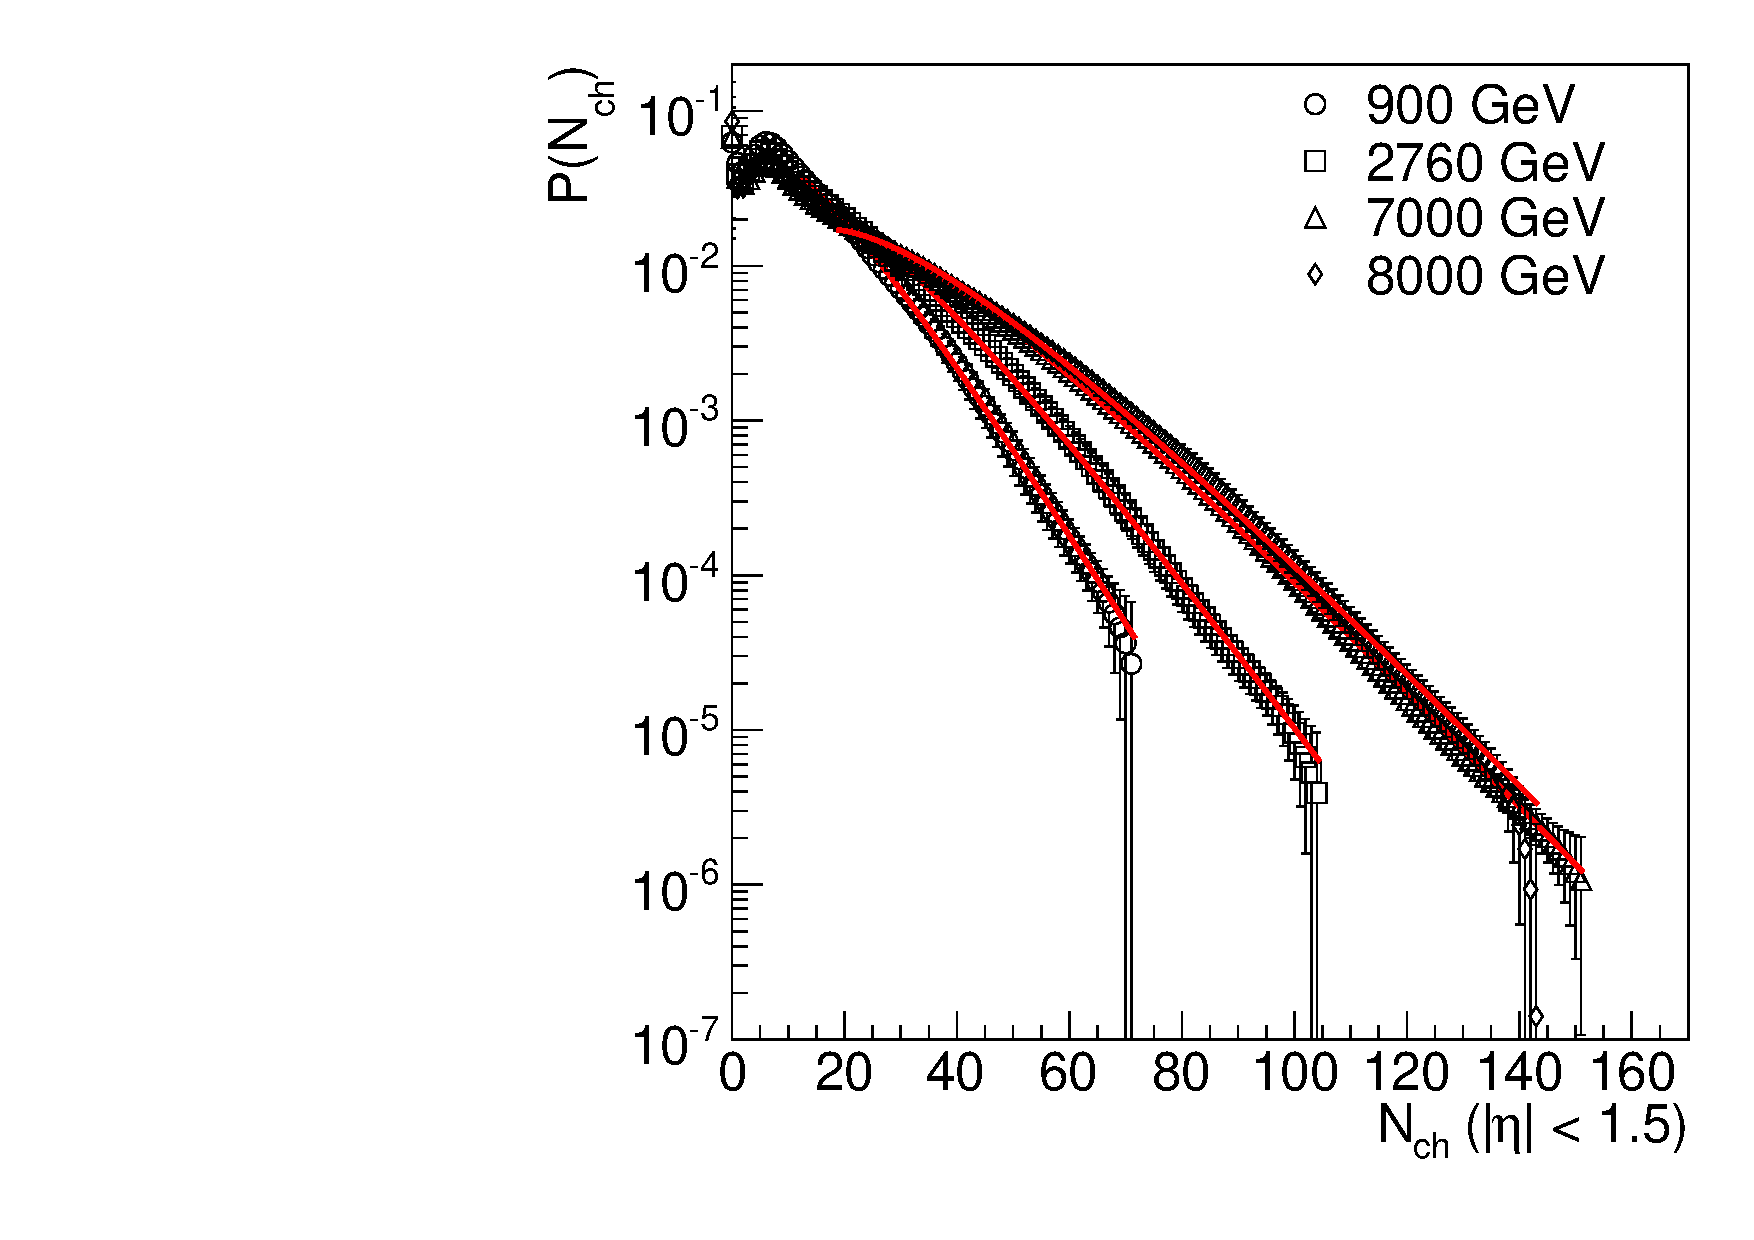
\includegraphics[width=0.49\linewidth]{\main/smallsystems/img/mult_data_1.pdf}
\hfill
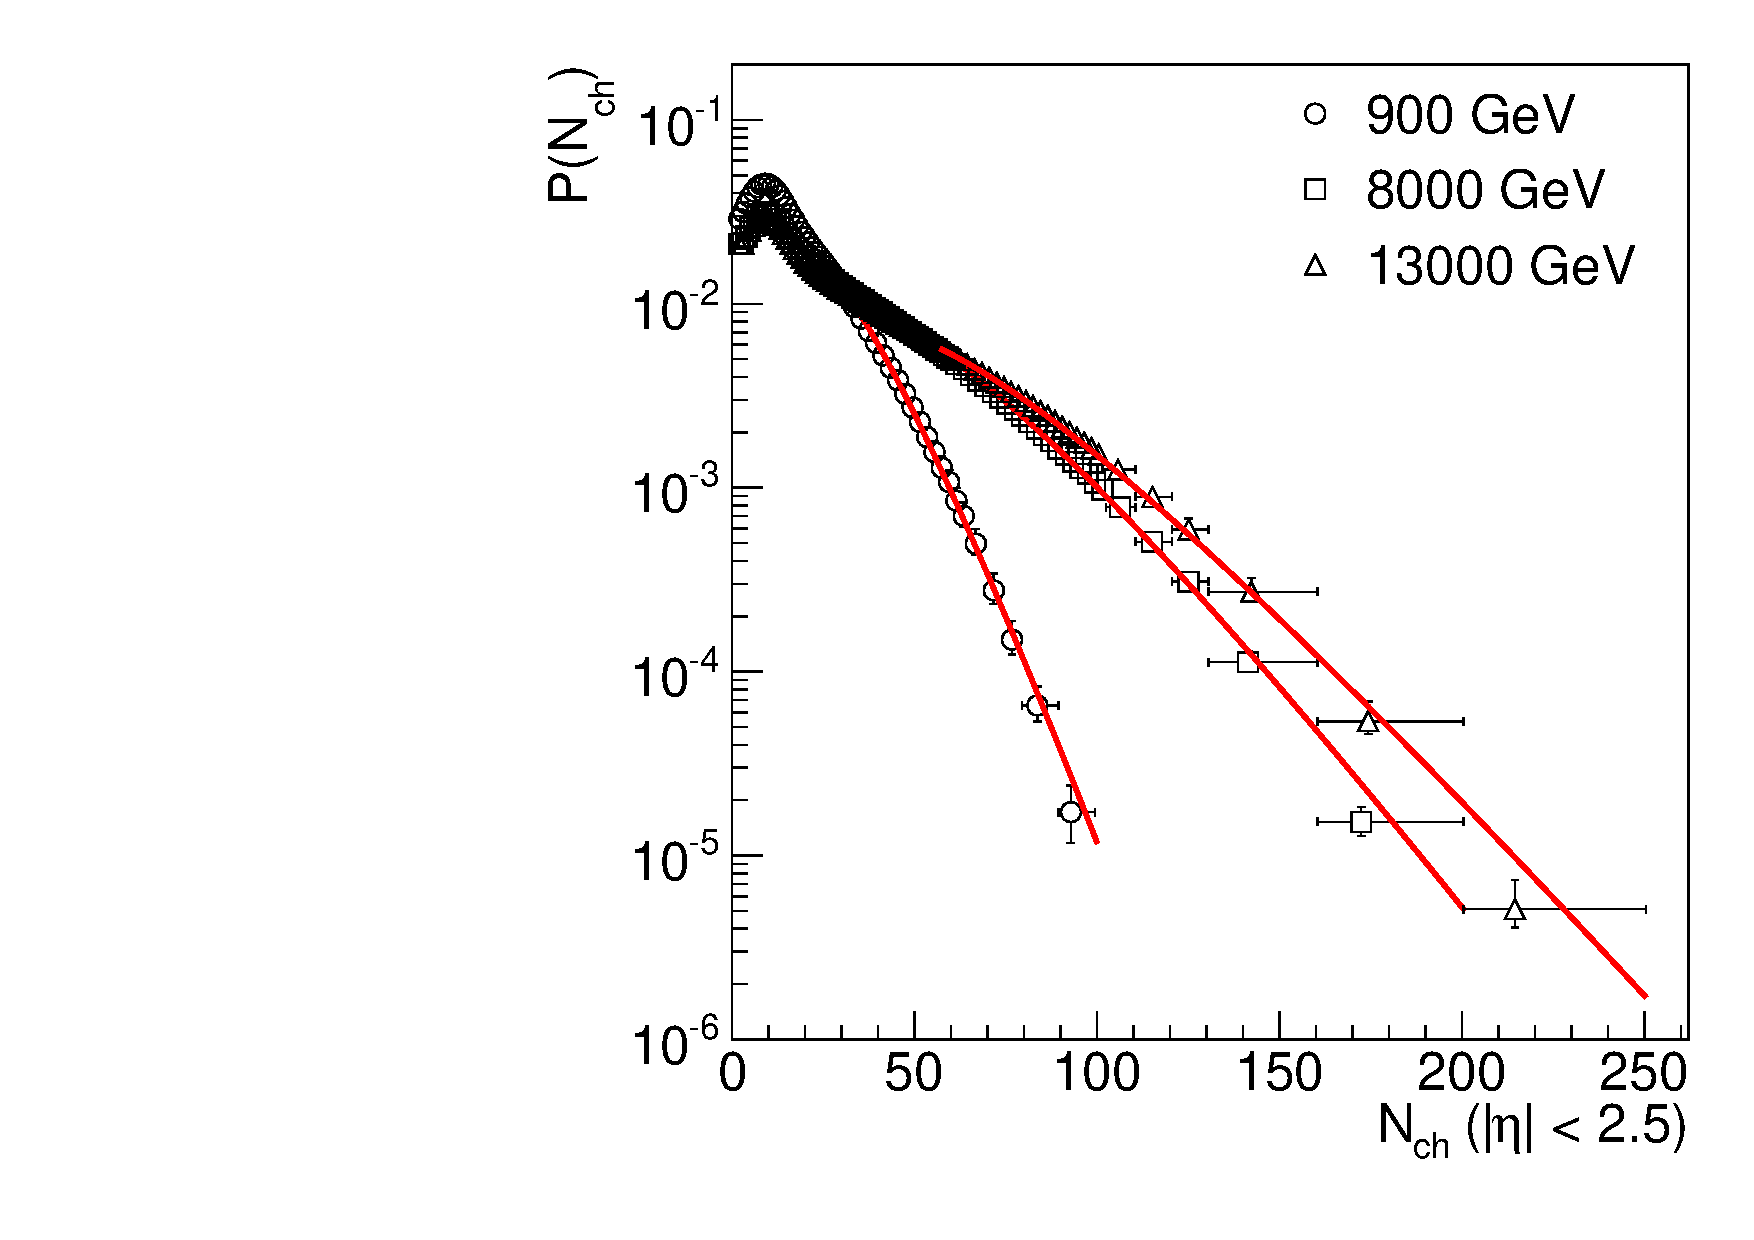
\includegraphics[width=0.49\linewidth]{\main/smallsystems/img/mult_data_11.pdf}
\caption{Multiplicity distributions measured by ALICE (left panel) and ATLAS (right panel) overlaid by the fit with a negative binomial distribution.}
\label{fig:smallsystems_mult_data}
\end{figure}

\begin{figure}[ht]
\centering
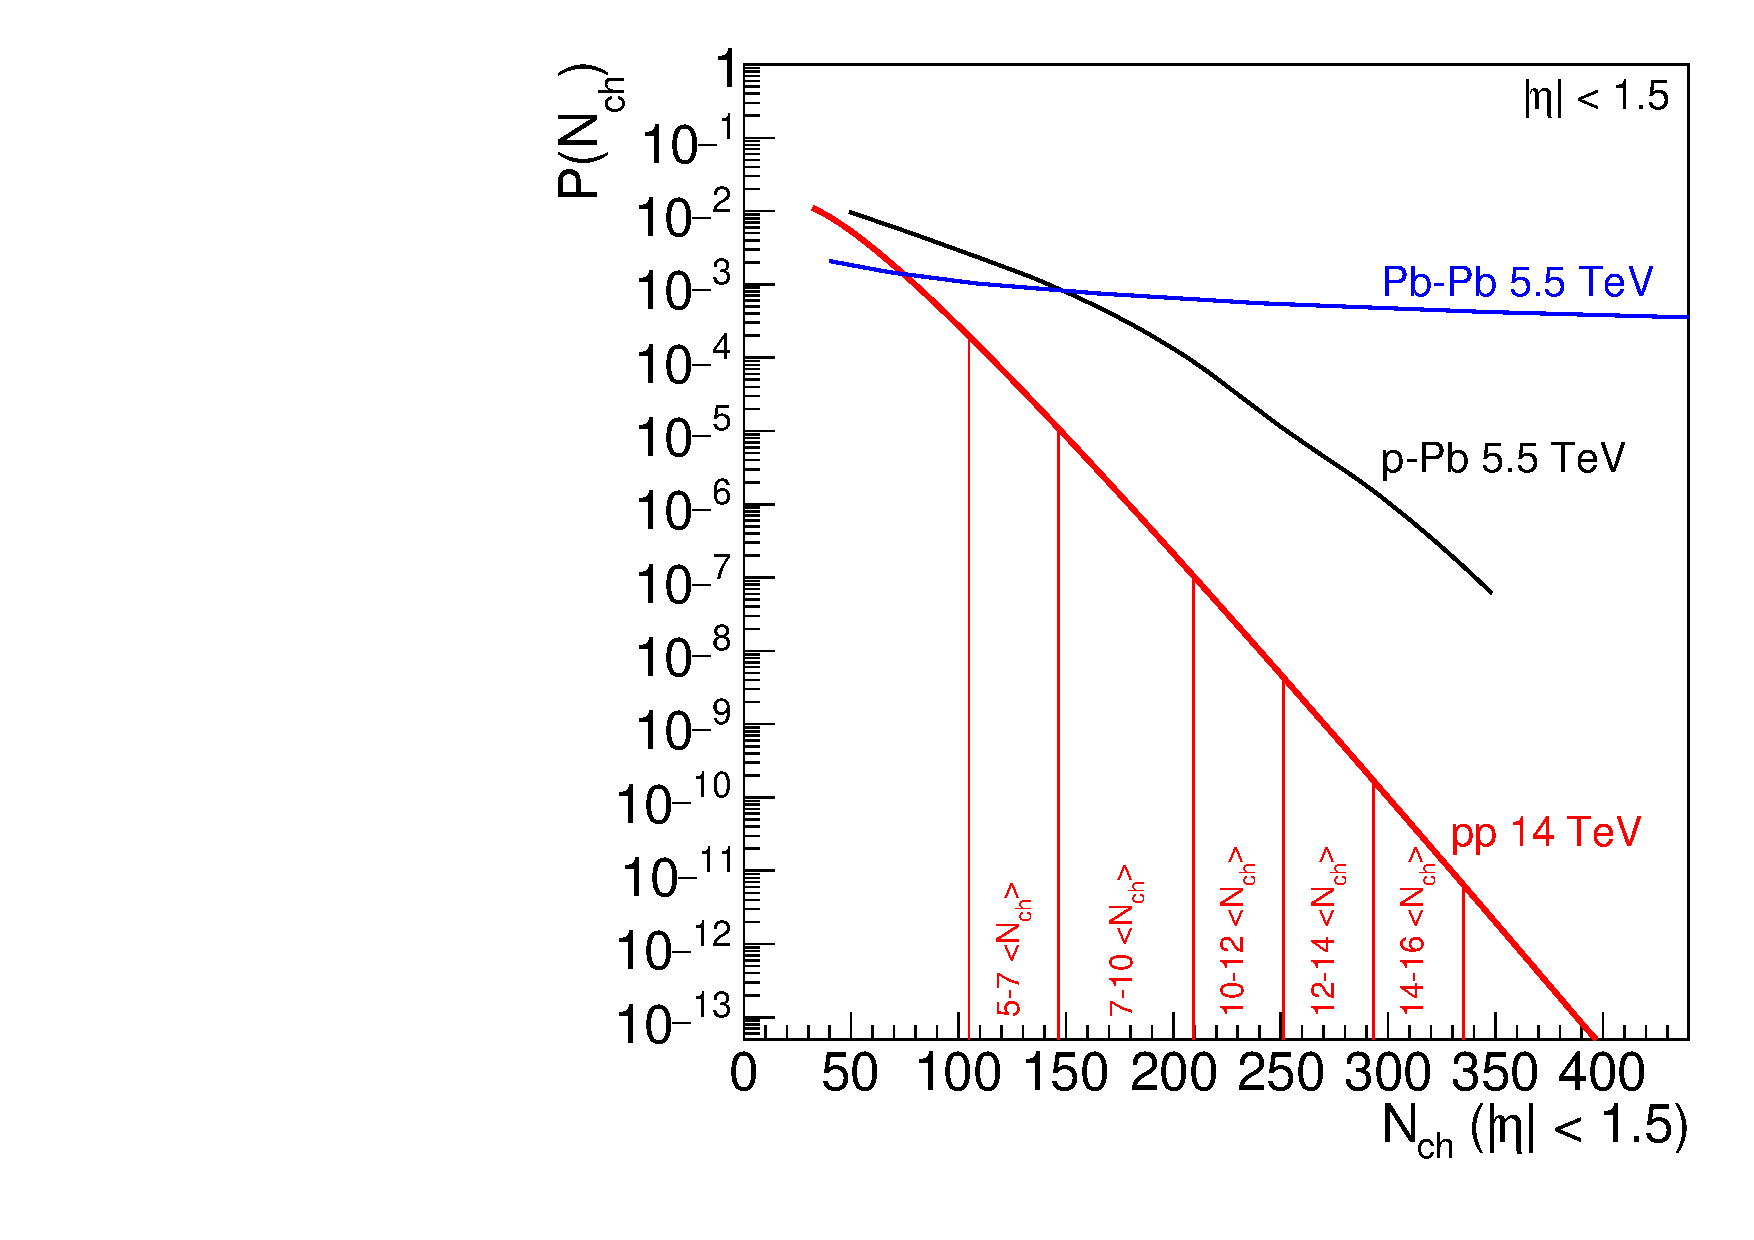
\includegraphics[width=0.32\linewidth]{\main/smallsystems/img/mult_extrapolation_alice.pdf}
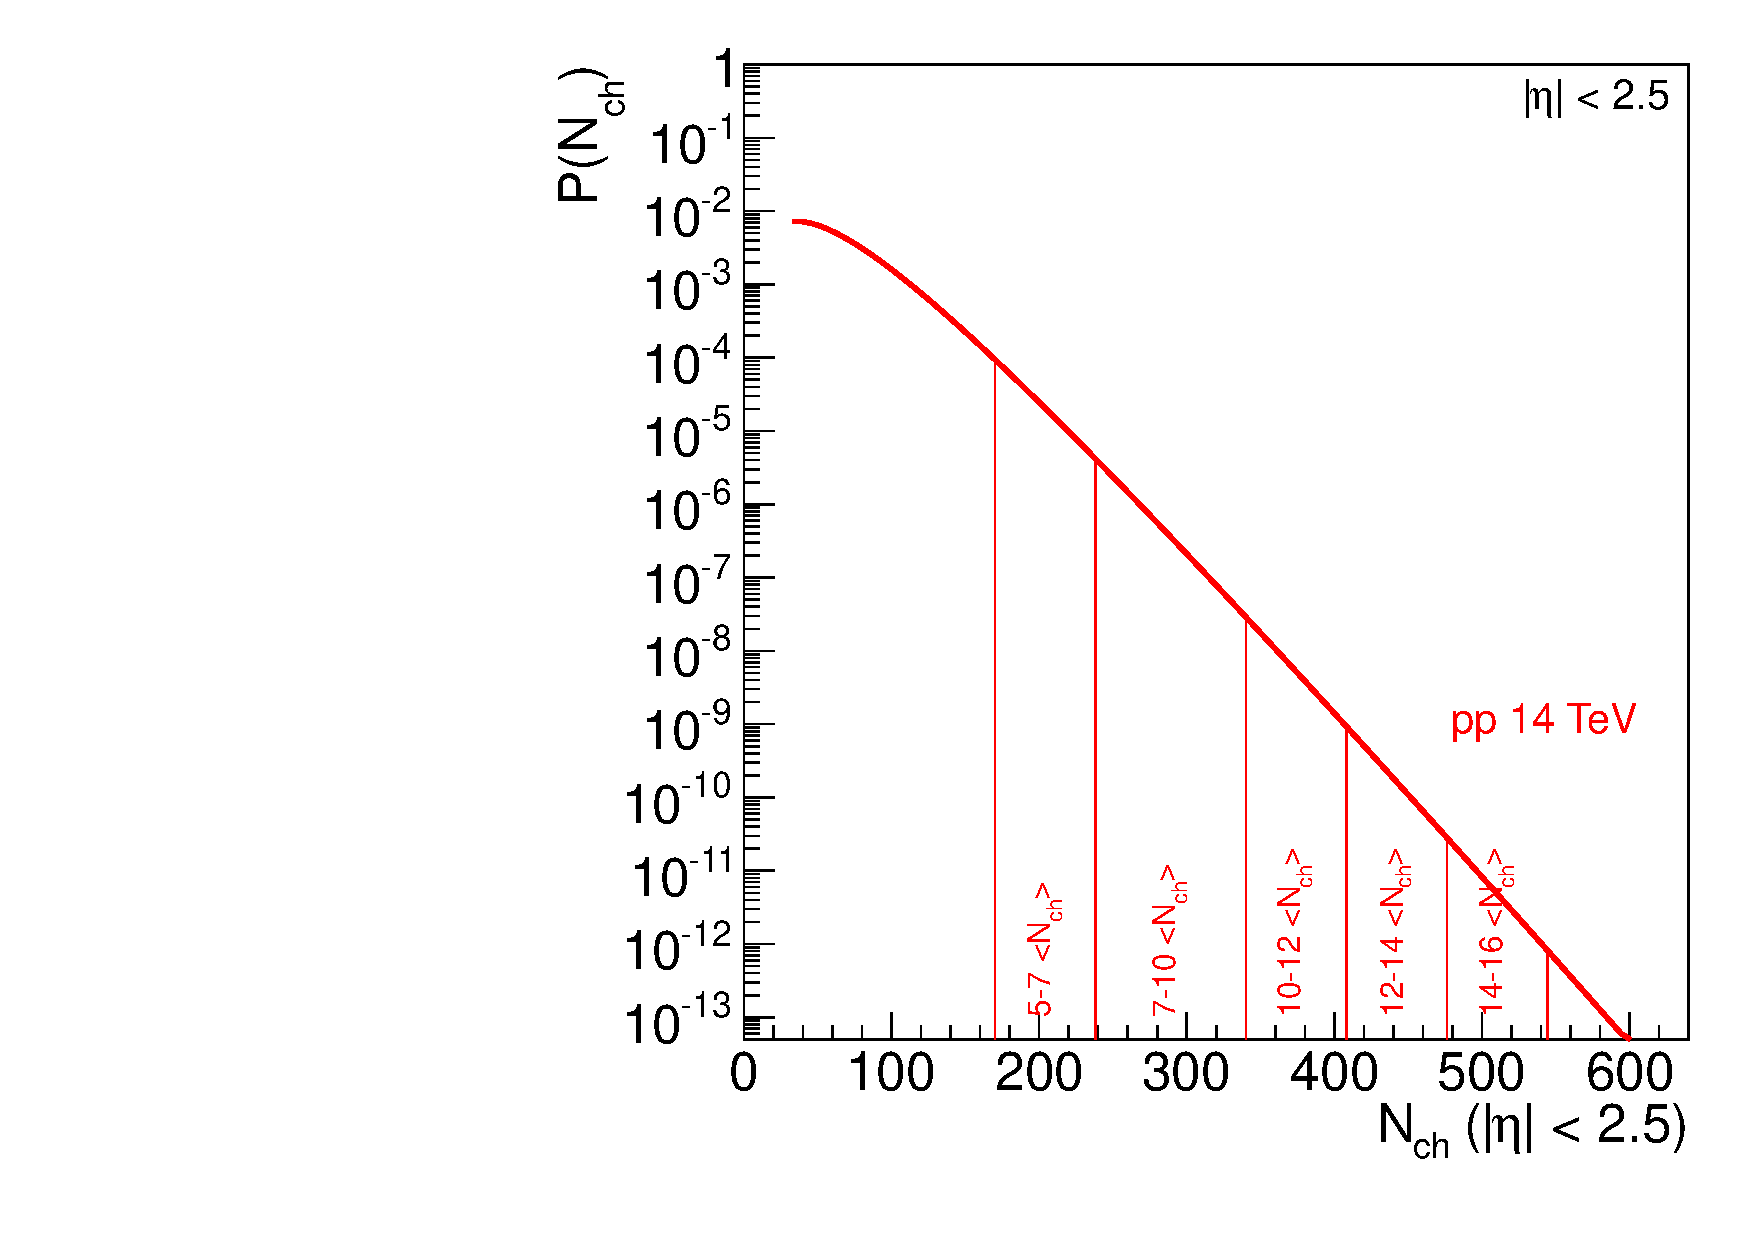
\includegraphics[width=0.32\linewidth]{\main/smallsystems/img/mult_extrapolation_atlas.pdf}
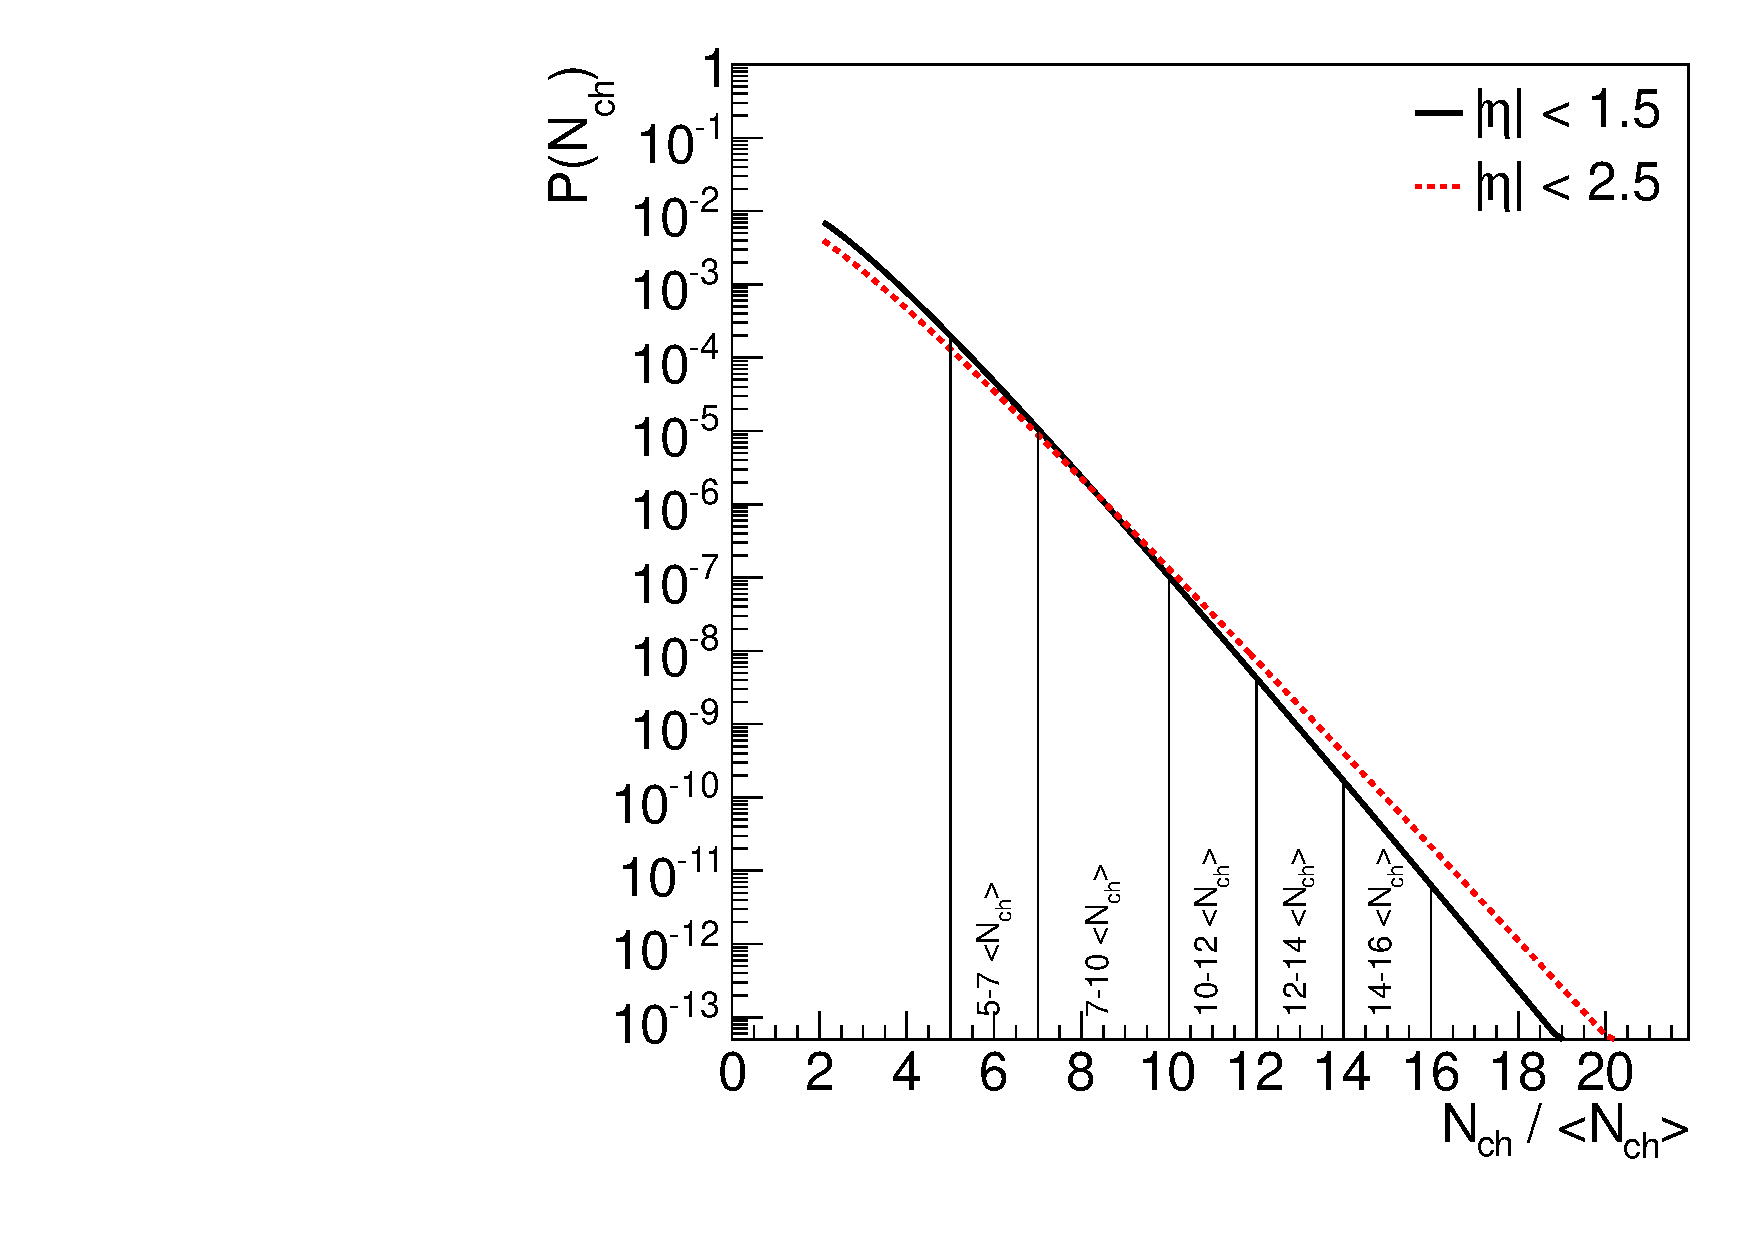
\includegraphics[width=0.32\linewidth]{\main/smallsystems/img/mult_extrapolation_comparison.pdf}
\caption{Extrapolated multiplicity distributions in pp collisions within $|\eta| < 1.5$ (left panel) and $|\eta| < 2.5$ (center panel). The indicated regions are from left to right for 5--7, 7--10, 10--12, 12--14, 14--16 times the average multiplicity. In the left panel the multiplicity distribution of Pb--Pb and p--Pb collisions is also plotted. The right panel compares these two distributions scaled by the average multiplicity. The extrapolation for $|\eta| < 2.5$ turns out to be a bit wider at large multiplicities; therefore the one based on $|\eta| < 1.5$ is used as baseline.}
\label{fig:smallsystems_mult_extrapolation}
\end{figure}

The resulting extrapolated multiplicity distribution for 14~TeV is shown in Fig.~\ref{fig:smallsystems_mult_extrapolation} for the ALICE and ATLAS case. In addition, these are compared scaled by their respective average multiplicities. The agreement is rather good, with some discrepancy in the tail of the distribution. The extrapolation based on the smaller phase space region falls off more quickly with multiplicity, and is therefore used as the more conservative estimate for all extrapolations.

Table~\ref{tab:smallsystems_pp} gives the fraction of cross-section and the number of events in 5 multiplicity classes:  5--7, 7--10, 10--12, 12--14 and 14--16 times the average multiplicity. Table~\ref{tab:smallsystems_pbpb} gives the number of events of bins with equivalent multiplicity than commonly measured multiplicity bins in p--Pb and Pb--Pb collisions. For the calculation of the number of events $\sigma_{\rm inel} = \unit[78.4]{mb}$ \cite{Loizides:2017ack} is used. These tables are the key input for the performance figures presented in this section. A high-multiplicity pp program sampling \unit[200]{pb$^{-1}$} is assumed for all experiments.
 
\begin{table}
\centering
\begin{tabular}{c|c|c|c|c}
Range & $\dNdeta$ & Fraction & Events per pb$^{-1}$ & Events in 200~pb$^{-1}$ \\
\hline
5--7 \nch     & 35--49   & 2.4e-03       & 1.9e+08       & 3.7e+10 \\
7--10 \nch    & 49--70   & 1.3e-04       & 1.0e+07       & 2.0e+09 \\
10--12 \nch   & 70--84   & 1.1e-06       & 9.0e+04       & 1.8e+07 \\
12--14 \nch   & 84--98   & 4.7e-08       & 3.7e+03       & 7.3e+05 \\
14--16 \nch   & 98--112  & 1.8e-09       & 1.4e+02       & 2.8e+04 \\
\hline
\end{tabular}
\caption{Number of pp events at 14 TeV in selected multiplicity bins.}
\label{tab:smallsystems_pp}
\end{table}

\begin{table}
\centering
\begin{tabular}{l|c|c|c}
Range & $\dNdeta$ & Events per pb$^{-1}$ & Events in 200~pb$^{-1}$ \\
\hline
0--5\% p--Pb   & 41--56        & 4.9e+07       & 9.8e+09 \\
5--10\% p--Pb  & 34--41        & 1.9e+08       & 3.8e+10 \\
10--20\% p--Pb & 27--34        & 6.6e+08       & 1.3e+11 \\
20--40\% p--Pb & 20--27        & 2.7e+09       & 5.4e+11 \\
\hline
60--65\% Pb--Pb    & 98--137       & 1.5e+02       & 3.0e+04 \\
65--70\% Pb--Pb    & 68--98        & 1.6e+05       & 3.1e+07 \\ 
70--75\% Pb--Pb    & 45--68        & 2.1e+07       & 4.2e+09 \\
75--80\% Pb--Pb    & 29--45        & 5.9e+08       & 1.2e+11 \\
80--85\% Pb--Pb    & 18--29        & 4.6e+09       & 9.1e+11 \\
\hline
\end{tabular}
\caption{Number of events in pp collisions at 14 TeV sliced in equivalent multiplicity bins as in p--Pb and Pb--Pb collisions.}
\label{tab:smallsystems_pbpb}
\end{table}

\subsubsection{Particle Correlations}

The measurements of two-particle correlations and higher-order cumulants have produced the initial observations of collectivity in small systems. In pp collisions, two distinct regions are of interest at HL-LHC: the high-multiplicity tail and the low-multiplicity regions. 

In pPb collisions, ...

The 4-particle cumulant is calculated for the third-order harmonics. Figure~\ref{fig:smallsystems_corr_cumulants} compares the $c_3\{4\}$ values between the published and the projected results, for $pp$ and $p$+Pb. In order to remove the non-flow contributions, 3-subevent method is applied. In the $pp$ collisions, with the data collected in Run 2, the statistical uncertainties are large and the $c_3\{4\}$ values are systematically consistent with zero in most $N_{ch}$ ranges. While in large systems, significant non-zero $c_3\{4\}$ has been measured, which reflects the fluctuation of triangle flow. Whether similar behavior is observed in small systems still needs to be confirmed. The increase in luminosity in Run 3 and Run 4 provides a great opportunity to measure $c_3\{4\}$ in $pp$ with high precision: the statistics are sufficient to measure down to $1.5\%$ $v_3\{4\}$ in the high multiplicity region. Similarly, in the $p$+Pb collision, the current result shows that $c_3\{4\}$ is consistent with zero, but increased statistics will help to detect potential non-zero $c_3\{4\}$ down to $1.5\%$ in most multiplicity ranges.

\begin{figure}[ht]
\centering
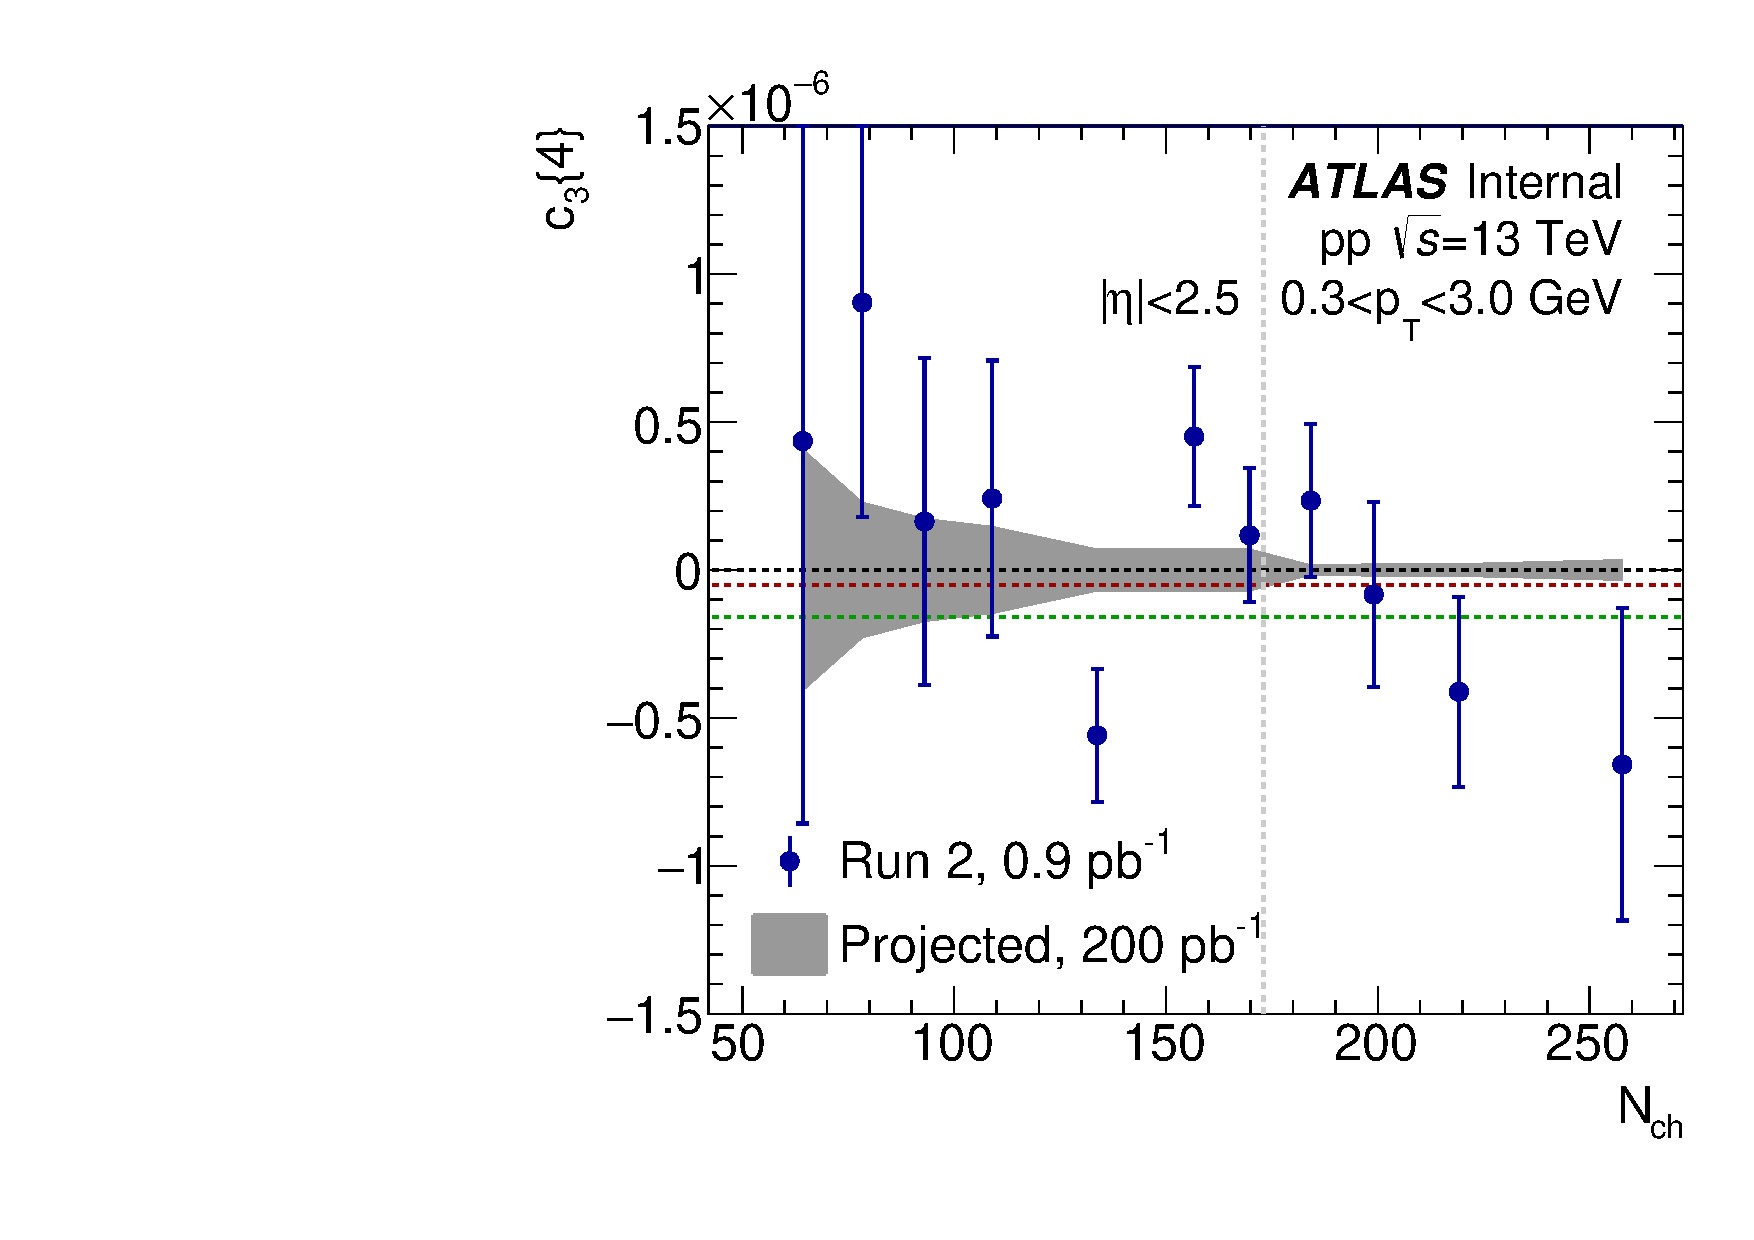
\includegraphics[width=.45\linewidth]{\main/smallsystems/img/c_3_4_pp.pdf}
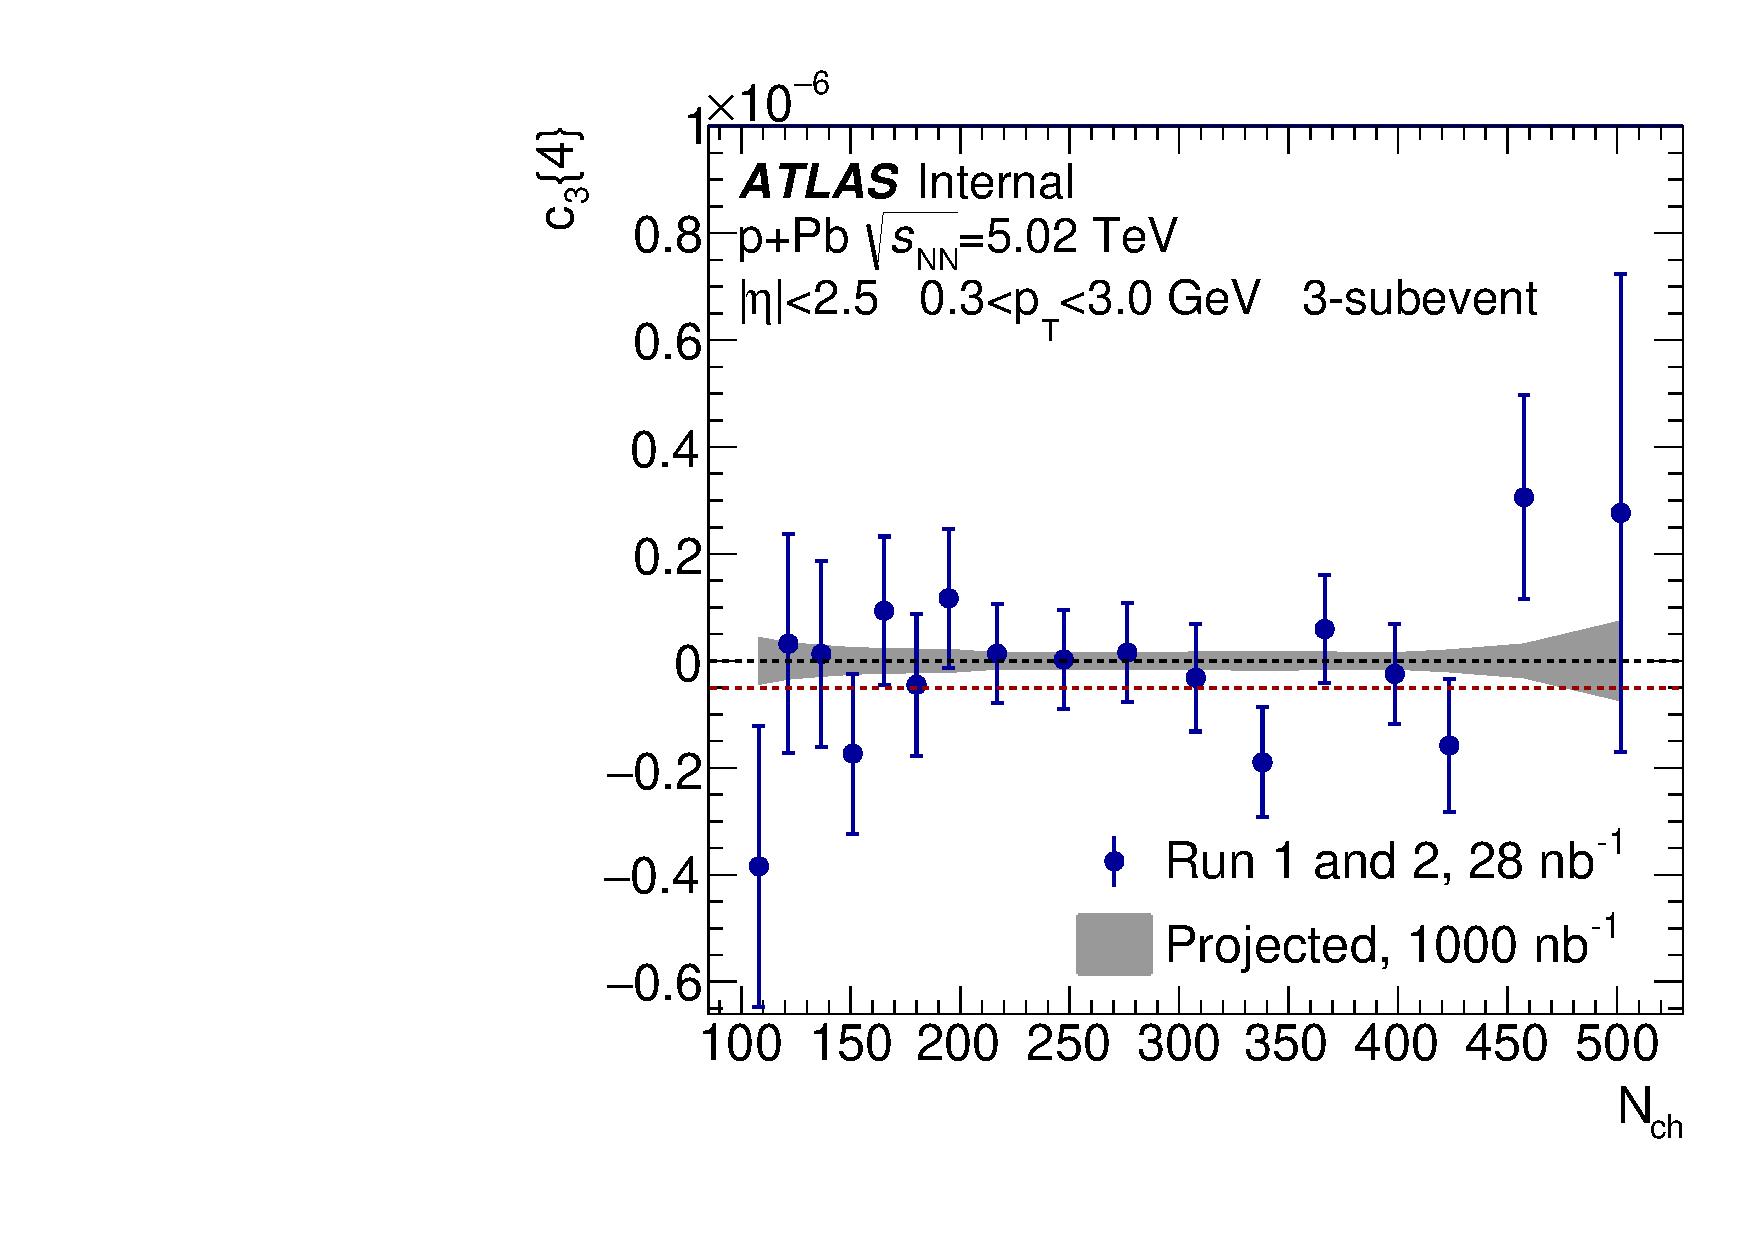
\includegraphics[width=.45\linewidth]{\main/smallsystems/img/c_3_4_pPb.pdf}
%\includegraphics[draft]{img/corr_cumulants.pdf}
\caption{4-particle cumulants $c_3\{4\}$ with 3-subevent method for $pp$ (left) and $p$+Pb (right) as a function of $N_{ch}$. Only statistical uncertainties are shown in the figure and the gray band represents the projected statistical uncertainty, with $c_3\{4\}$ assumed to be zero. The red and green dash lines represent $1.5\%$ and $2.0\%$ $v_3\{4\}$ signal respectively.}
\label{fig:smallsystems_corr_cumulants}
\end{figure}

\begin{figure}[ht]
\centering
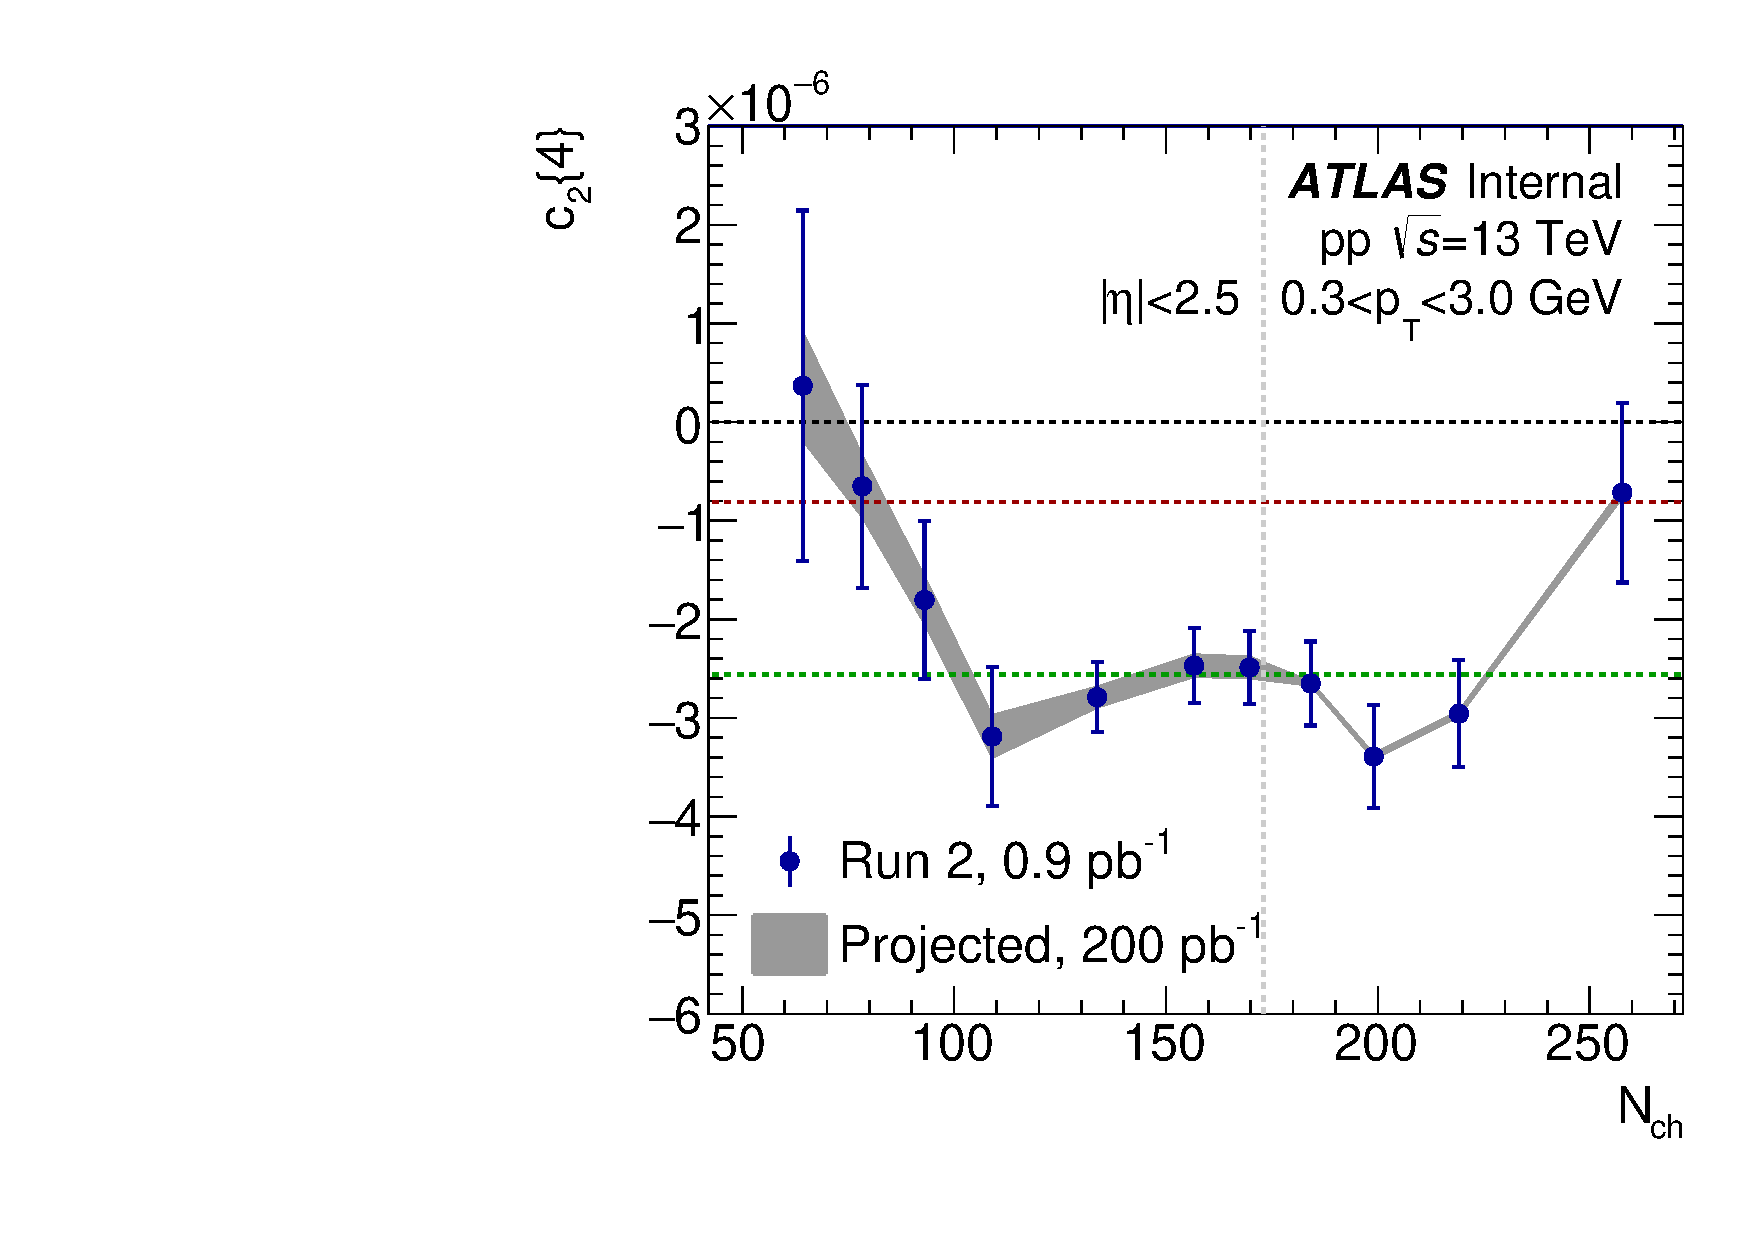
\includegraphics[width=.45\linewidth]{\main/smallsystems/img/c_2_4_pp.pdf}
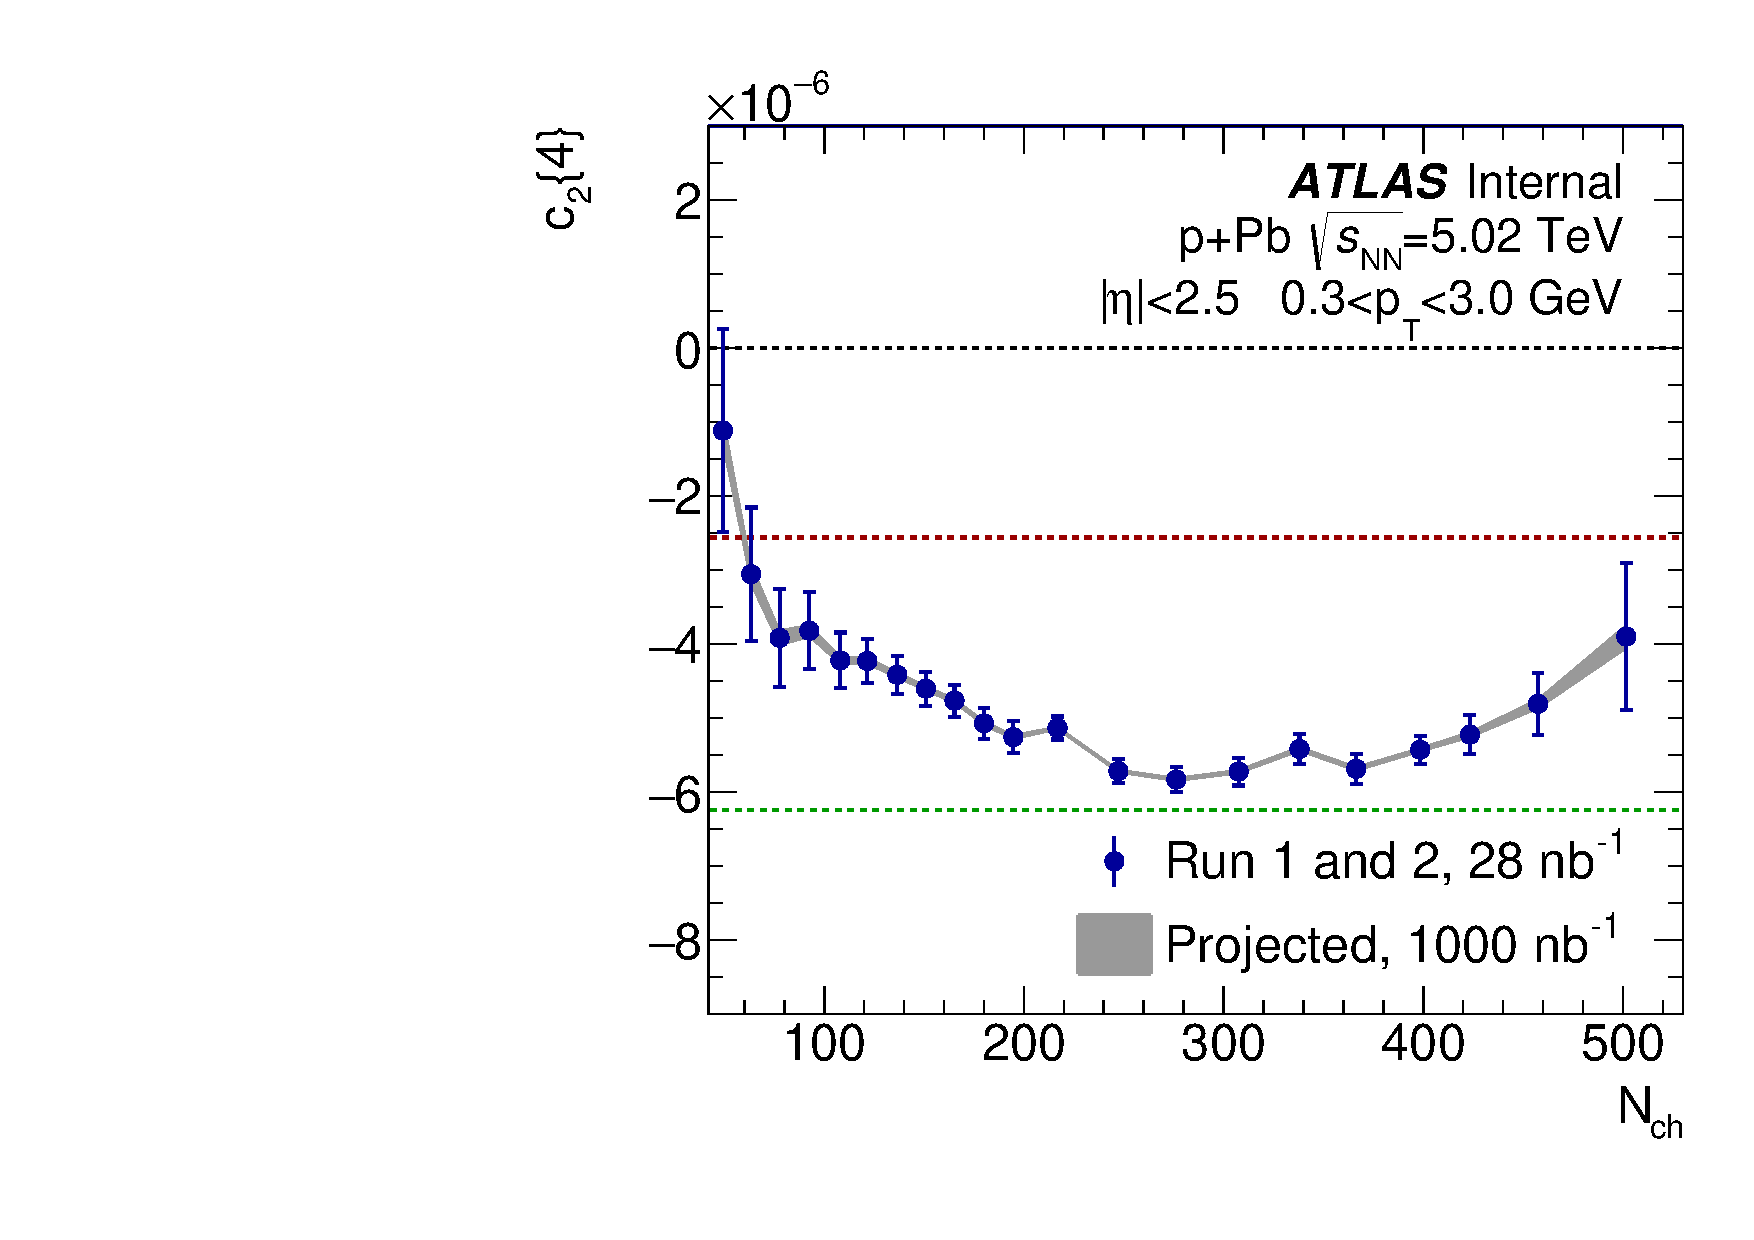
\includegraphics[width=.45\linewidth]{\main/smallsystems/img/c_2_4_pPb.pdf}
%\includegraphics[draft]{img/corr_cumulants.pdf}
\caption{4-particle cumulants $c_2\{4\}$ with 3-subevent method for $pp$ (left) and $p$+Pb (right) as a function of $N_{ch}$. Only statistical uncertainties are shown in the figure and the gray band represents the projected statistical uncertainty. The red and green dash lines represent $3\%$ and $4\%$ $v_2\{4\}$ signals for $pp$, and $4\%$ and $5\%$ $v_2\{4\}$ signals for $p$+Pb.}
\label{fig:smallsystems_corr_cumulants_v2}
\end{figure}



\begin{figure}[ht]
\centering
\includegraphics[draft]{\main/smallsystems/img/corr_symmetriccumulants.pdf}
%\includegraphics[draft]{img/corr_symmetriccumulants.pdf}
\caption{Symmetric cumulants extracted with and without applying subevents for pp (left) and pPb (right) as a function of Nch. CMS.}
\label{fig:smallsystems_corr_symmetriccumulants}
\end{figure}

\begin{figure}[ht]
\centering
\includegraphics[draft]{\main/smallsystems/img/corr_cumulants_pid.pdf}
%\includegraphics[draft]{img/corr_cumulants_pid.pdf}

\caption{Particle identified $v_n$ (TODO only v2?) coefficients for pi, K, p (pp, ALICE), D mesons (pp, CMS), J/Psi (pp, pPb, ALICE, CMS) as a function of pT. Note that the multiplicity ranges are different for the different estimates. TODO: Plot may be messy and may need splitting in several panels.}
\label{fig:smallsystems_corr_cumulants_pid}
\end{figure}

\begin{figure}[ht]
\centering
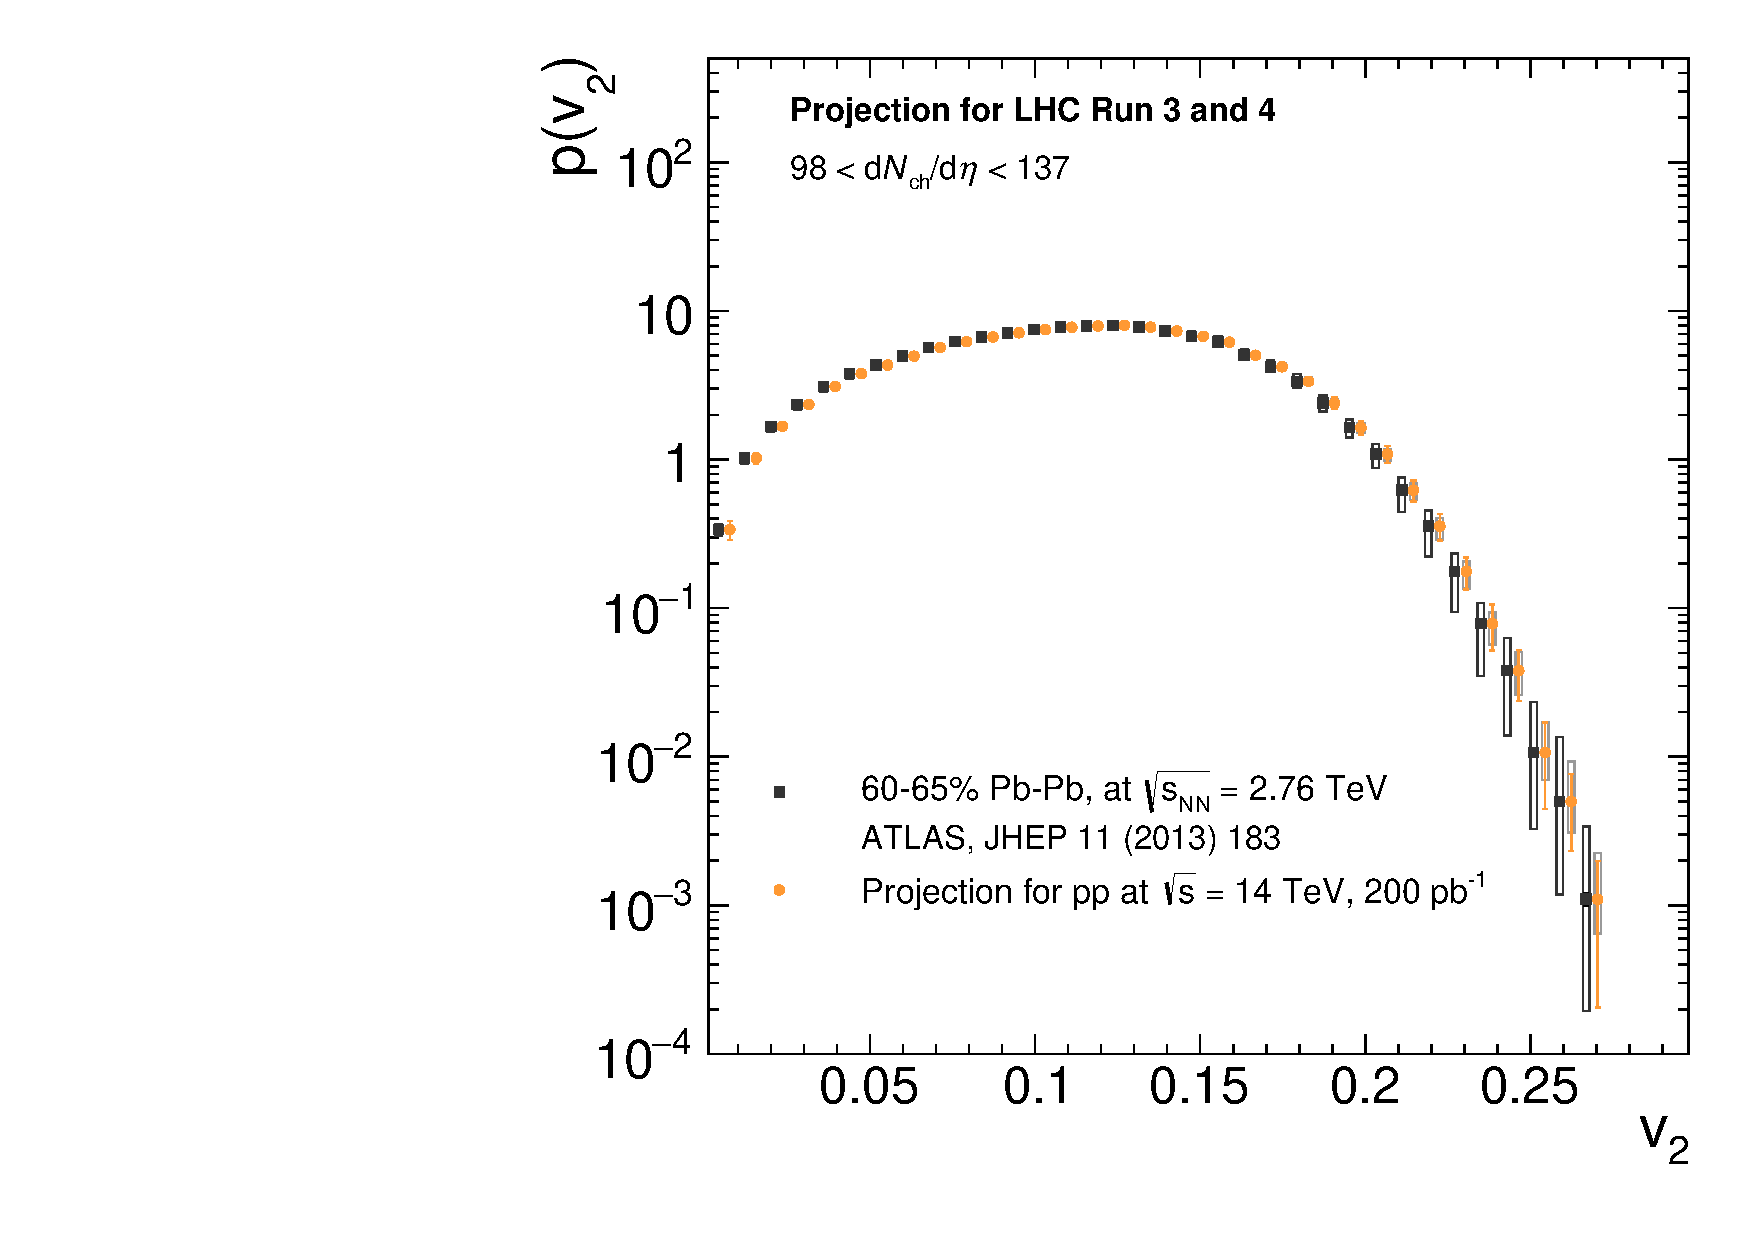
\includegraphics[width=.49\linewidth]{\main/smallsystems/img/ebye_v2_60-65_276TeVppprojection.pdf}

\caption{Projection of the measurement of the probability distribution of $v_2$ in pp collisions. To illustrate the reach the same signal as in Pb--Pb is assumed. The projection is for the equivalent pp multiplicity (circles) to 60--65\% centrality in Pb--Pb collisions (squares).}
\label{fig:smallsystems_corr_pvn}
\end{figure}

\subsubsection{Strangeness Enhancement}

\begin{figure}[ht]
\centering
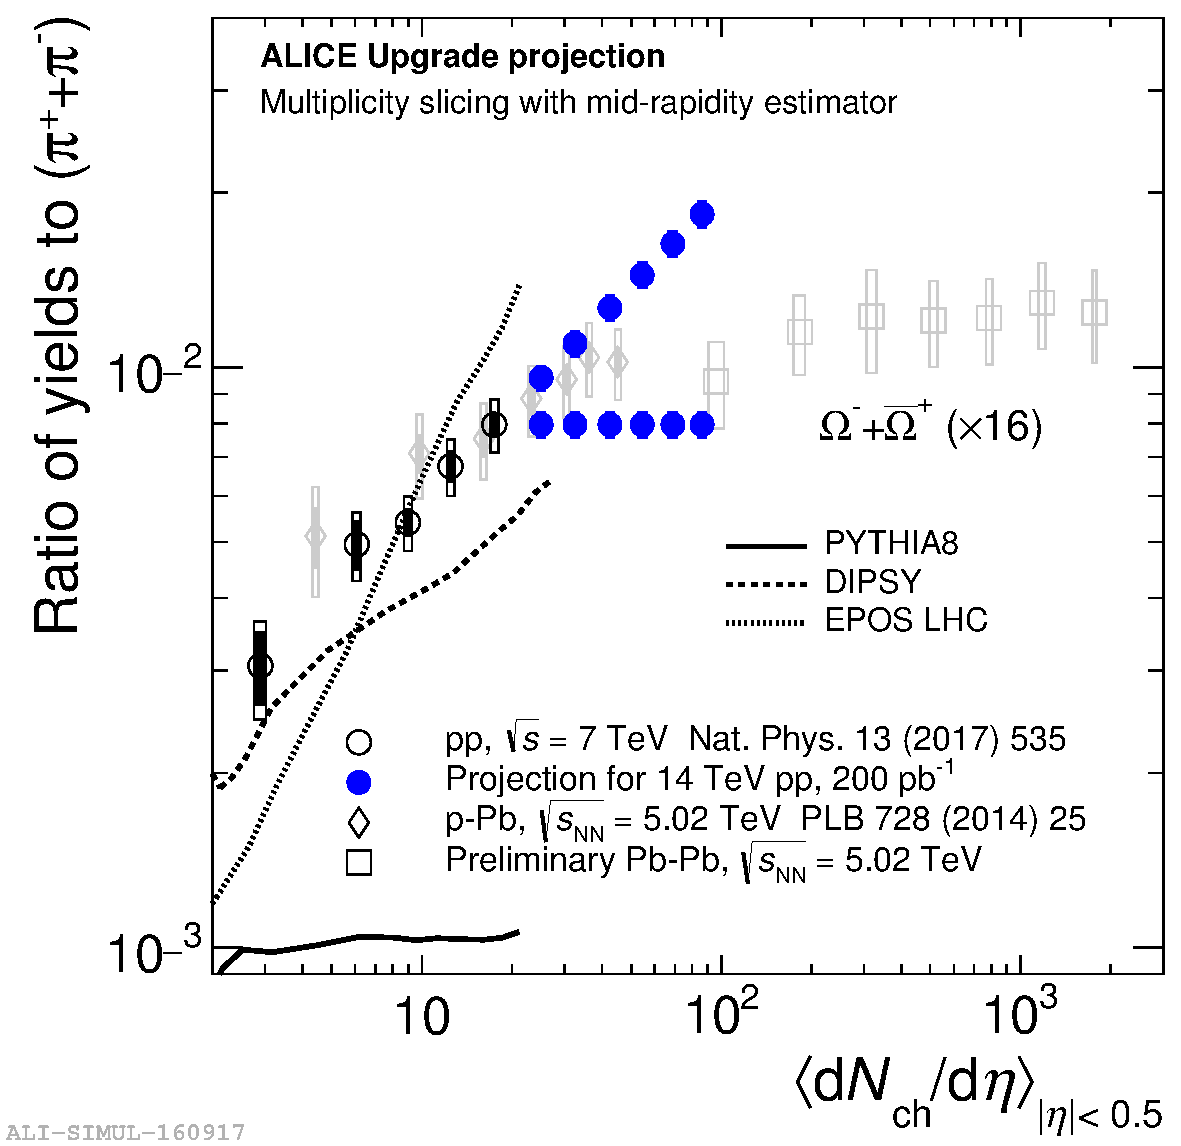
\includegraphics[width=0.49\linewidth]{\main/smallsystems/img/strangeness_omegapi.pdf}

\caption{$\Omega/\pi$ ratio as a function of $\nch$ for pp, p--Pb, and Pb--Pb collisions. The existing data (from Ref.~\cite{ALICE:2017jyt}) is shown in open black symbols, the extrapolation for pp collision is denoted by blue filled circles.}
\label{fig:smallsystems_strangeness_omega_pi}
\end{figure}

\subsubsection{Energy Loss}

Narrative: 
- Existing pA eloss measurements (ALICE, ATLAS, CMS) show limit of maximal few percent quenching. In conclusion, RpA is not a good observable
- Produce estimates for a) h-jet (a la ALICE), b) gamma-jet or Z-jet (ATLAS/CMS), c) jet substructure
- Produce these for pA and pp
- For pp, see if high mu sample can be also used for something. In fact it should be made clear where it can be used and where not, as this chapter will be one of the places where a low mu pp program is motivated.

\begin{figure}[ht]
\centering
\includegraphics[draft]{\main/smallsystems/img/energyloss_hjet.pdf}
%\includegraphics[draft]{img/energyloss_hjet.pdf}
\caption{Modification of jet recoil yields extracted from hadron-jet correlations for pp collisions (left) and p-Pb collisions (right). Delta-recoil ratio vs. pT.}
\label{fig:smallsystems_energyloss_hjet}
\end{figure}

\begin{figure}[ht]
\centering
\includegraphics[draft]{\main/smallsystems/img/energyloss_Zjet.pdf}
%\includegraphics[draft]{img/energyloss_Zjet.pdf}

\caption{Z-jet correlations in pp (left panel) and p-Pb collisions (right panel). 1/N dN/dxZj vs xZj.}
\label{fig:smallsystems_energyloss_Zjet}
\end{figure}

\subsubsection{Thermal Radiation}

\begin{figure}[ht]
\centering
\includegraphics[draft]{\main/smallsystems/img/thermal_radiation.pdf}
\caption{Thermal dileptons. Left panel: dN/Mee vs. Mee Example. Right panel: sensitivity as a function of Lint (pp, pPb) [expected signal is too uncertain].}
\label{fig:smallsystems_thermal_radition}
\end{figure}

\subsection{Data-taking strategy}

% High multiplicity triggering, pile up, MB sample
% pp
%   ALICE: additional several month pp program
%   ATLAS/CMS: special runs (mu~1) or special conditions at end of fill
%   LHCb: either in nominal (mu~5) or special running
%   HM sample: 200 pb-1 pp (per experiment)
%   How much MB for low-multiplicity questions?
% p-Pb scheduled run
%   1000-2000 nb-1

\subsection{Summary}

\clearpage

\bibliographystyle{report}   % Remember we use title in the biblio
\bibliography{bib/section}

\end{document}
